%% Classe du document
\documentclass[a4paper,10pt]{article}

%% Francisation
\usepackage[english]{babel} % Indique que l'on utilise le francais
\usepackage[T1]{fontenc}
\usepackage[utf8]{inputenc} % Indique que l'on utilise tout le clavier
%\usepackage[latin1]{inputenc}

%% Réglages généraux
\usepackage[top=2.3cm, bottom=2.3cm, left=3cm, right=3cm]{geometry} % Taille de la feuille
\usepackage{lastpage}

%% Package pour le texte
\usepackage{soul} % Souligner
\usepackage{color} % Utilisation de couleurs
\usepackage{hyperref} % Créer des liens et des signets
\usepackage{eurosym}% Pour le symbole euro
\usepackage{fancyhdr}% Entête et pied de page

%% Package pour les tableaux
\usepackage{multirow} % Colonnes multiples
\usepackage{cellspace}
\usepackage{array}

%% Package pour les dessins
\usepackage{pstricks}
\usepackage{graphicx} % Importer des images
\usepackage{pdftricks} % Pour utiliser avec pdfTex
\usepackage{pst-pdf} % Pour utiliser avec pdfTex
\usepackage{pst-node} % Pose de noeuds
\usepackage{subfig}
\usepackage{float}

%% Package pour les maths
\usepackage{amsmath} % Commandes essentielles
\usepackage{amssymb} % Principaux symboles

%% Package pour le code
\usepackage{listings} % Utilisation de la couleur syntaxique des langages
\usepackage{url}


\usepackage[babel=true]{csquotes} % Permet les quotations (guillemets)
\usepackage{tocvsec2}
\usepackage{amsthm}
\usepackage{amsfonts}

\usepackage{tikz}
\usepackage{pdfpages}

\usetikzlibrary{shapes} % A revoir

%--------------------- Autres définitions ---------------------%

% Propriété des liens
\hypersetup{
colorlinks = true, % Colorise les liens
urlcolor = blue, % Couleur des hyperliens
linkcolor = black, % Couleur des liens internes
}

\definecolor{grey}{rgb}{0.95,0.95,0.95}

% Language Definitions for Turtle
%TODO: a revoir avec les couleur de gedit
\definecolor{olivegreen}{rgb}{0.2,0.8,0.5}
\definecolor{grey2}{rgb}{0.5,0.5,0.5}
\lstdefinelanguage{ttl}{
sensitive=true,
morecomment=[s][\color{grey2}]{@}{:},
morecomment=[l][\color{olivegreen}]{\#},
morecomment=[s][\color{red}]{<}{/>},
morestring=[s][\color{olivegreen}]{<http://w}{\#>},
morestring=[b][\color{blue}]{\"},
}

\lstset{
frame=single,
breaklines=true,
basicstyle=\ttfamily,
backgroundcolor=\color{grey},
basicstyle=\scriptsize,
keywordstyle=\color{blue},
commentstyle=\color{green},
stringstyle=\color{red},
identifierstyle=\color{blue}
}

%Definition de la commande pour retirer l'espace devant les ':'
\makeatletter
\@ifpackageloaded{babel}%
        {\newcommand{\nospace}[1]{{\NoAutoSpaceBeforeFDP{}#1}}}%  % !! double {{}} pour cantonner l'effet à l'argument #1 !!
        {\newcommand{\nospace}[1]{#1}}
\makeatother

\setcounter{tocdepth}{3}
%\maxsecnumdepth{subsubsection} % Dernière section numérotée

\newcommand{\paperPrototyping}{\emph{paper prototyping}}

% Corps du document :
\begin{document}

% Définition des entêtes et pieds de page
\fancyhead[LE,CE,RE,LO,CO,RO]{}
\fancyfoot[LE,CE,RE,LO,CO,RO]{}
\fancyhead[LO, LE]{English}
\fancyhead[RO,RE]{2012/2013}
\fancyfoot[LO,LE]{Université de \scshape{Nantes}}
\fancyfoot[RO,RE]{Page \thepage \ sur \pageref{LastPage}}
\renewcommand{\headrulewidth}{0.4pt}
\renewcommand{\footrulewidth}{0.4pt}

%\maketitle
\begin{titlepage}

\vspace*{\fill}~
\begin{center}
{\large \textsc{Guide}} \\
\vspace{1cm}
{\LARGE How to create a beautiful blog} \\
\vspace{1cm}
COUTABLE Guillaume, MENORET Clément, RULLIER Noémie, WOLLENBURGER Antoine \\
\today
\end{center}
\vspace*{\fill}

\vspace{\stretch{1}}
\begin{center}
\noindent 

\includegraphics[height=2.5cm]{Images/universite.png}
\end{center}
\pagebreak
\end{titlepage}

\newpage
\tableofcontents 

% Introduction
\newpage
\pagestyle{fancy}

%TODO : Correction des fautes d'orthographes, tournures de phrases ... en continu
%TODO : En fonction des parties de tous le monde redire à Nomyx de diminuer ses images pour pas que ça dépasse 10 page (environ) --> arg ! c'est pas assez 10 pages

%%%%%%%%%%%%%%%%%%%%%%%%%%%%%%%%%%%%%%%%%%%%%%%%%%%%%%%%%%%%%%%%%%%%%%%%%%%%%
%%%%%%%%%%  Introduction générale
%%%%%%%%%%%%%%%%%%%%%%%%%%%%%%%%%%%%%%%%%%%%%%%%%%%%%%%%%%%%%%%%%%%%%%%%%%%%%
\section{Introduction}

There are a lot of tools available to create a blog. They are addressed to different persons from novice to professional.

This document is a tutorial to help you to create your own blog. We consider that you are not an expert, that's why we choose a tool designed for anyone: \emph{Overblog}.

To practice this tutorial, you need an internet connection and a valid email address.

%%%%%%%%%%%%%%%%%%%%%%%%%%%%%%%%%%%%%%%%%%%%%%%%%%%%%%%%%%%%%%%%%%%%%%%%%%%%%
%%%%%%%%%%  Etape 1
%%%%%%%%%%%%%%%%%%%%%%%%%%%%%%%%%%%%%%%%%%%%%%%%%%%%%%%%%%%%%%%%%%%%%%%%%%%%%
\newpage
\section{Sign up on overblog}
The first step is to sign up on overblog. Let's see how to do this:
\begin{enumerate}
\item First, open your web browser (for example \emph{Internet Explorer} 
\includegraphics[width=0.5cm]{Images/explorer.png} or \emph{Google chrome} 
\includegraphics[width=0.5cm]{Images/chrome.png}).
\item Go on \emph{Google}, type \emph{overblog} in the search bar and validate. Then click on this link:
\begin{figure}[H]
    \center
	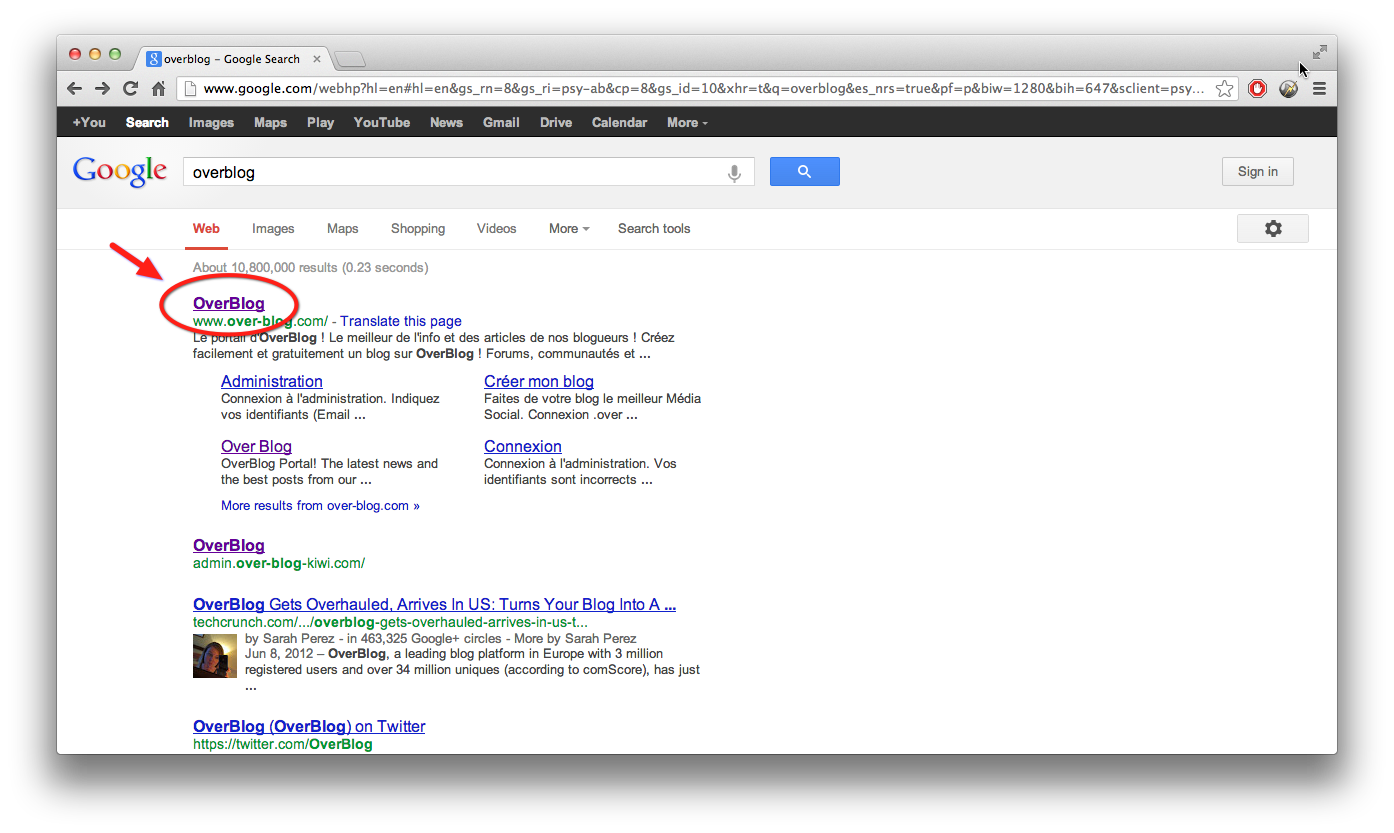
\includegraphics[width=13cm]{Images/linkOverblog.png}
    \caption{Overblog's link}
\end{figure}
Or you can also type in your adress bar this link \url{http://en.over-blog.com/}
\item Now, you have to sign up. Go at the bottom of the page and click on \emph{Sign up now} like this:
\begin{figure}[H]
    \center
	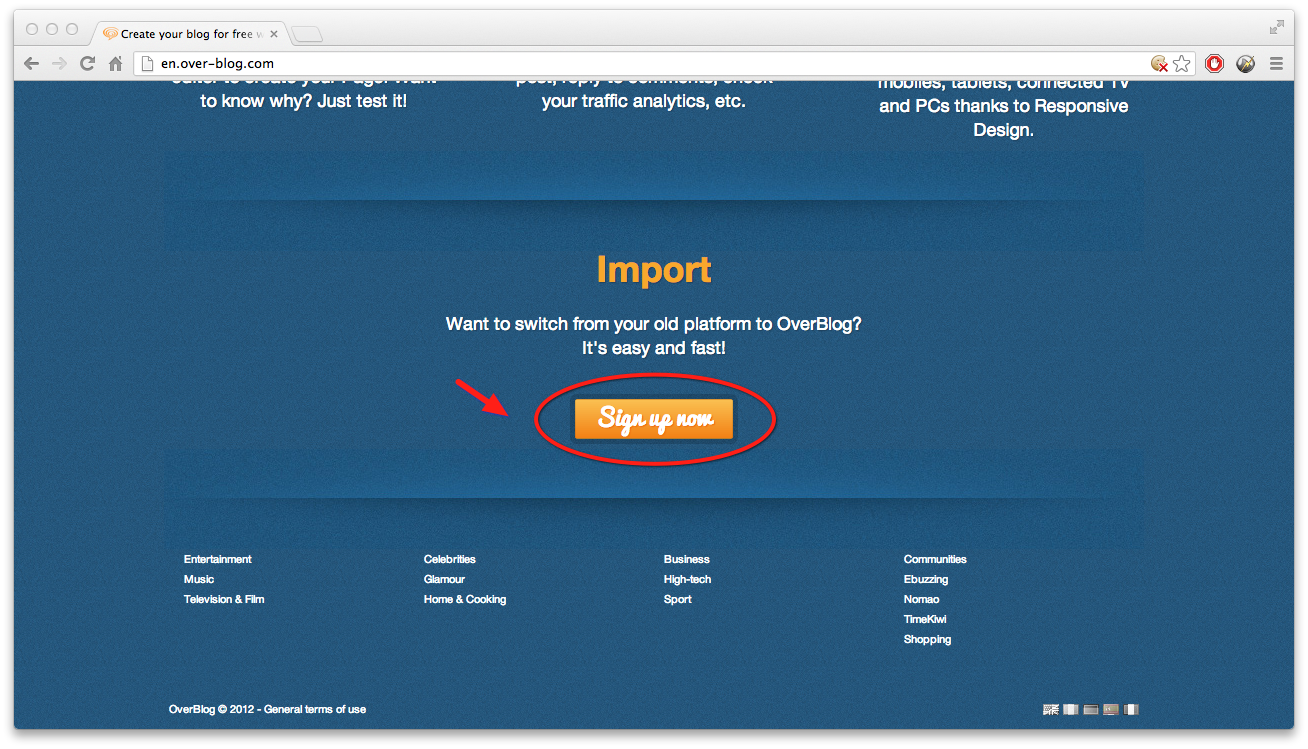
\includegraphics[width=13cm]{Images/signUpButton.png}
    \caption{Sign up button}
\end{figure}
\item Then you are redirected to this page:
\begin{figure}[H]
    \center
	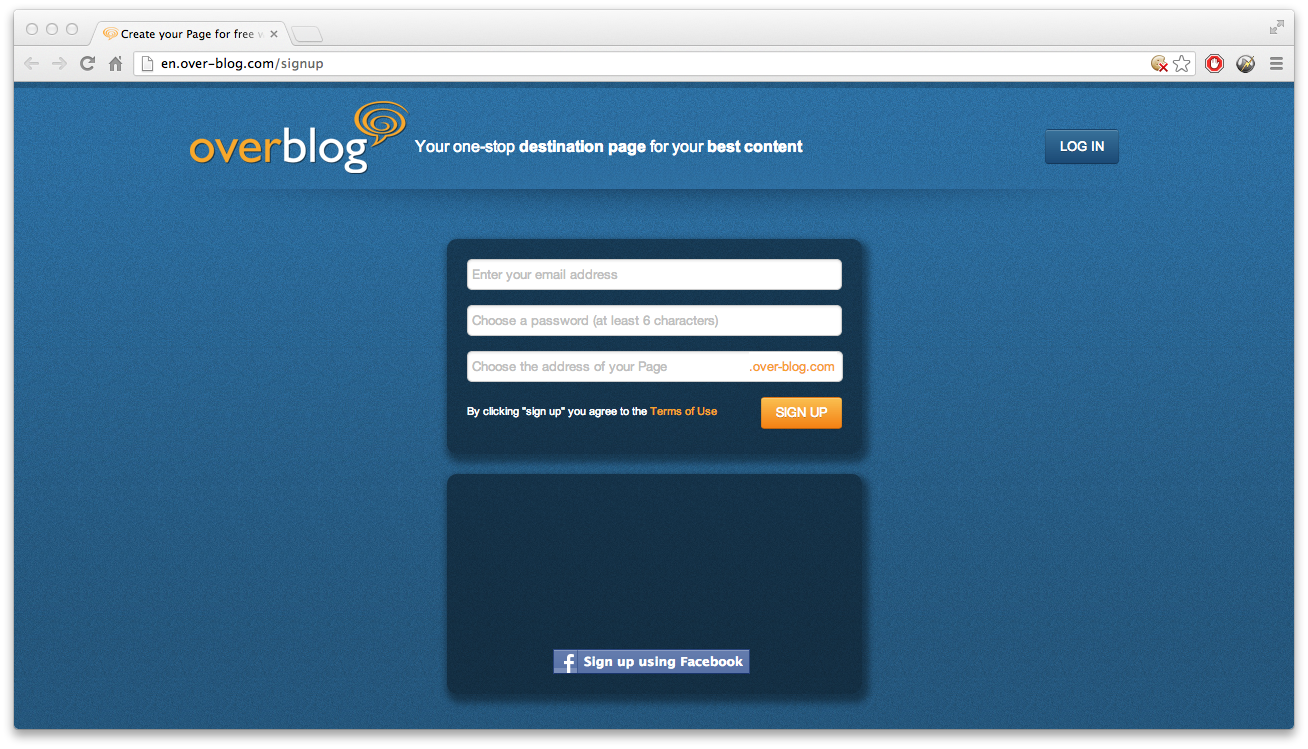
\includegraphics[width=13cm]{Images/signUpPage.png}
    \caption{Sign up page}
\end{figure}
You have to provide a valid email address because in the next step you have to confirm your registration by clicking a link wich is send on it. Moreover, you have to enter a password and the begining of the address you want for your blog (you have no choice for the end of the address, it must end with \emph{.over-blog.com}. Here is an example:
\begin{figure}[H]
    \center
	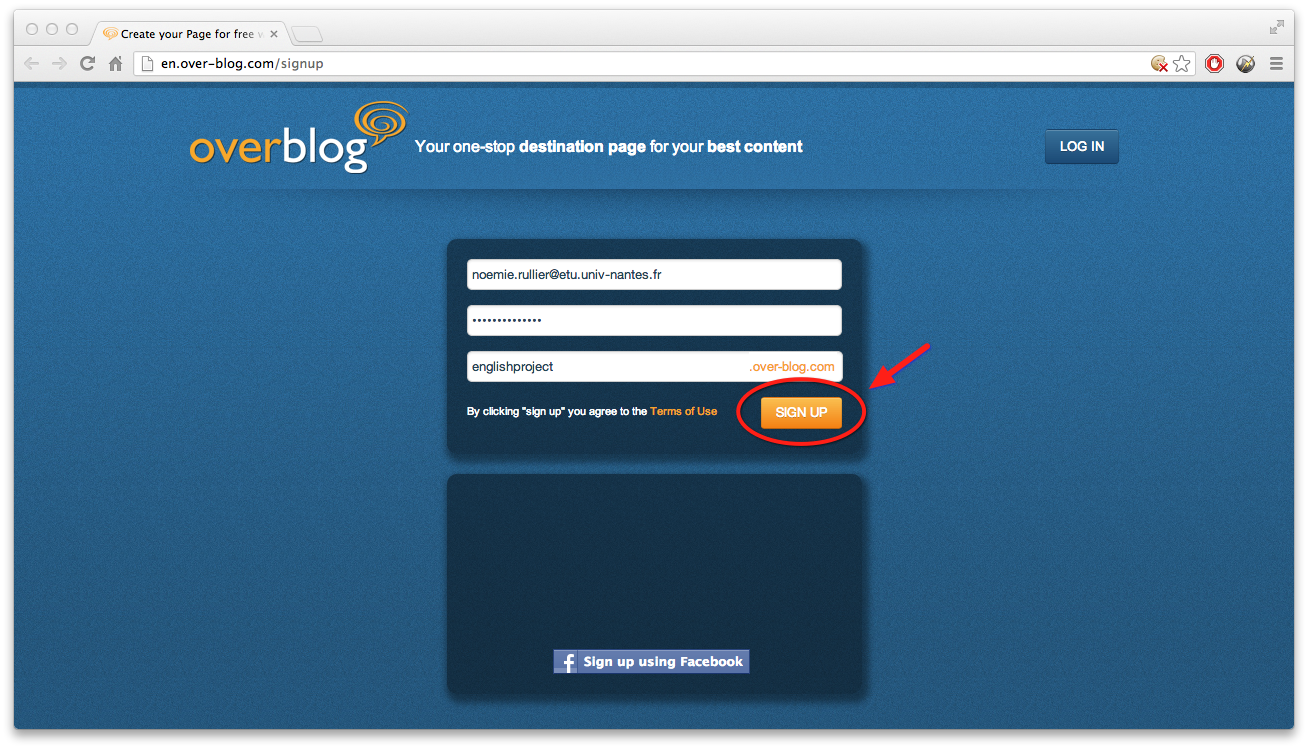
\includegraphics[width=13cm]{Images/signUpPageValues.png}
    \caption{Sign up page with values}
\end{figure}
Then click on \emph{SIGN UP}.
\item Then you are redirected on this page:
\begin{figure}[H]
    \center
	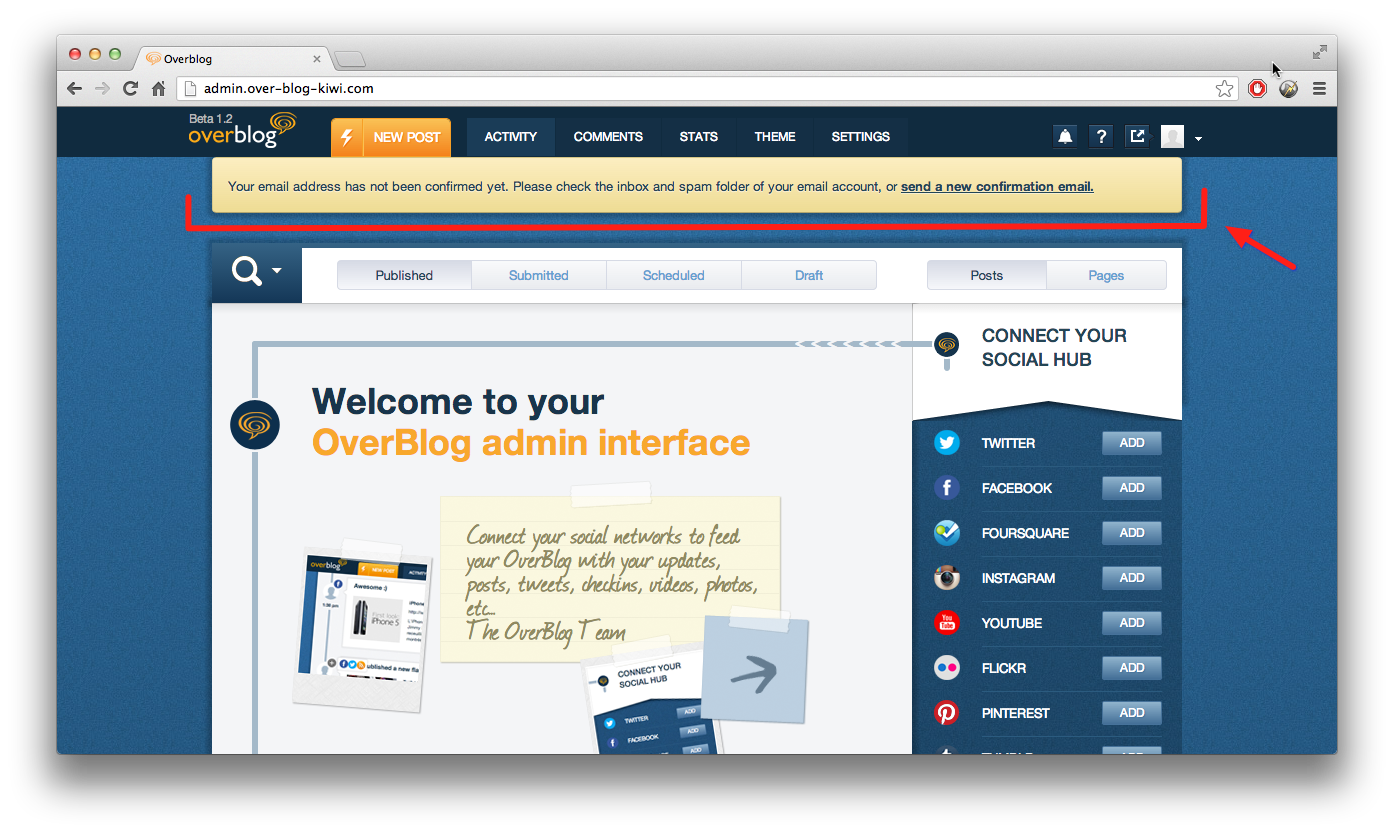
\includegraphics[width=13cm]{Images/addressMailNotConfirmed.png}
    \caption{Email address not confirmed}
\end{figure}
You can see that you have not confirmed your email address yet. Open your personal information manager, and open the mail sent by \emph{marie@overblog.com}. If you don't see this mail, refresh your email box or look for it in your spam folder. The mail should look like that: 
\begin{figure}[H]
    \center
	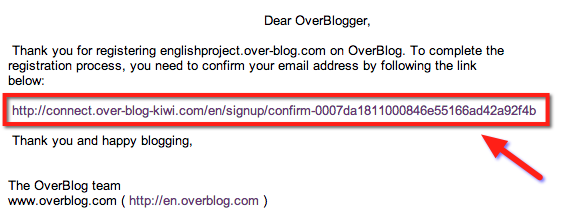
\includegraphics[width=10cm]{Images/emailOverblog.png}
    \caption{Email send by overblog}
\end{figure}
Click on the link surrounded in red. You will be redirected on this page:
\begin{figure}[H]
    \center
	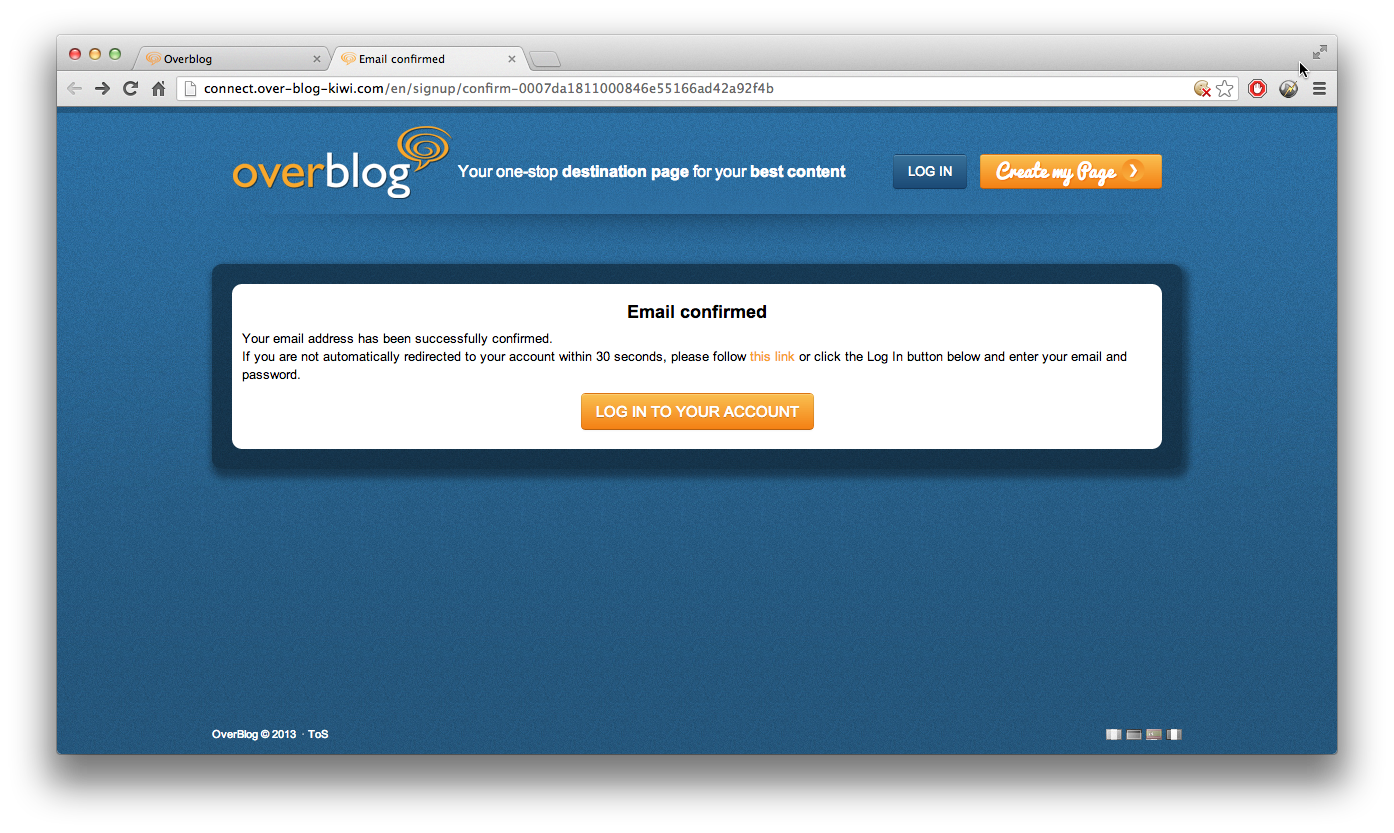
\includegraphics[width=13cm]{Images/addressMailConfirmed.png}
    \caption{Email address confirmed}
\end{figure}
To confirm the validation of your account, you are redirected to this page:
\begin{figure}[H]
    \center
	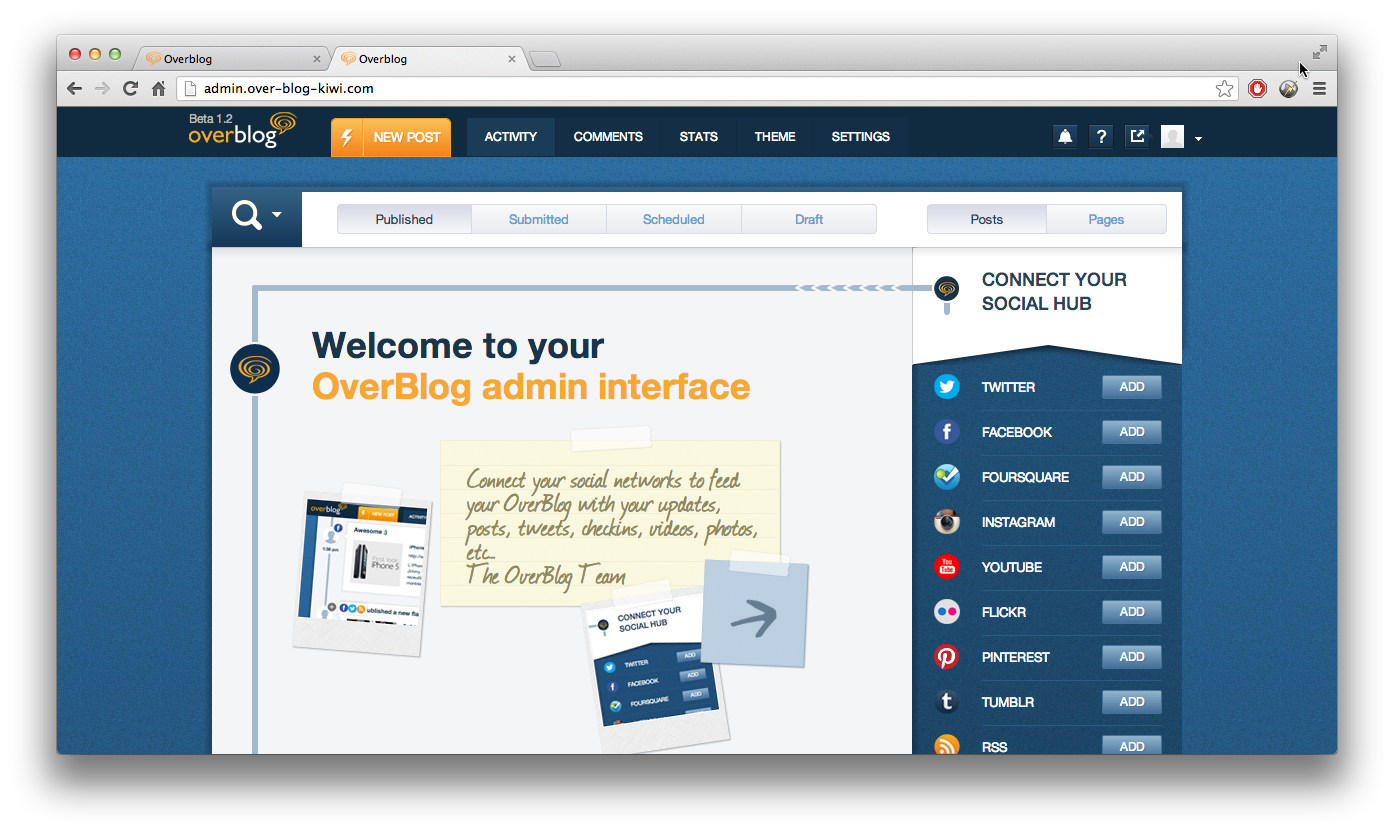
\includegraphics[width=13cm]{Images/overblogPage.png}
    \caption{Overblog's home page}
\end{figure}
You are now ready to use your blog !
\end{enumerate}


%%%%%%%%%%%%%%%%%%%%%%%%%%%%%%%%%%%%%%%%%%%%%%%%%%%%%%%%%%%%%%%%%%%%%%%%%%%%%
%%%%%%%%%%  Etape 2
%%%%%%%%%%%%%%%%%%%%%%%%%%%%%%%%%%%%%%%%%%%%%%%%%%%%%%%%%%%%%%%%%%%%%%%%%%%%%
\newpage
\section{Create an article}

Now that you got your own blog set up, let's add some content ! 

\subsection{Textual content}

\subsubsection{Posting}

\begin{figure}[H]
    \center
	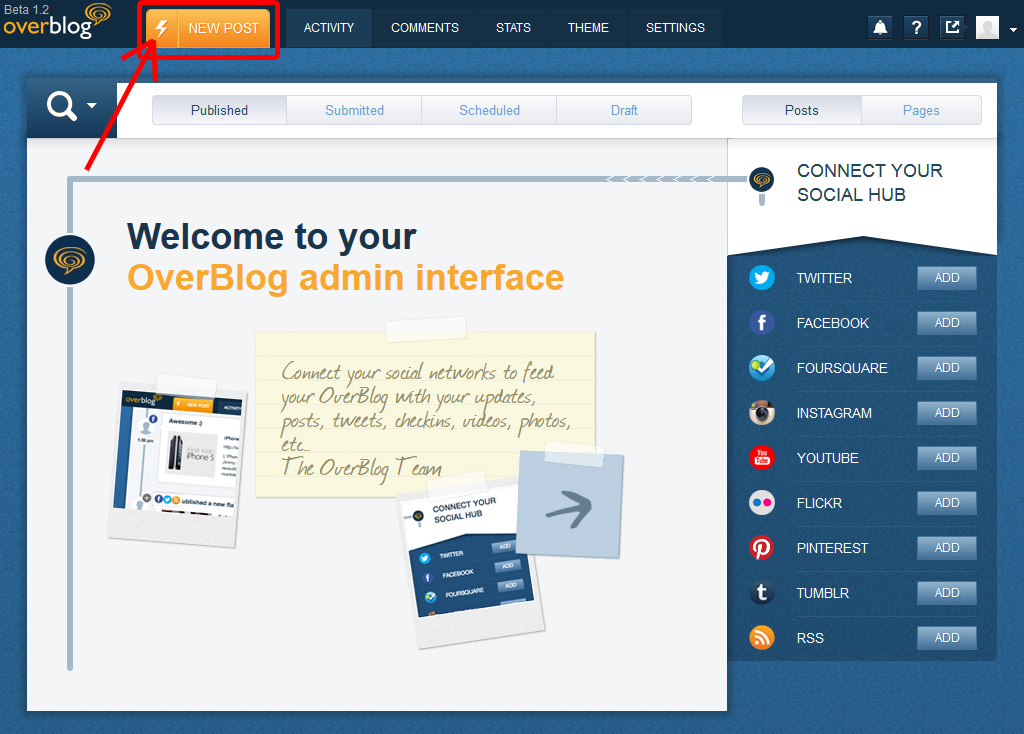
\includegraphics[width=13cm]{Images/strike001.png}
    \caption{The flash icon will allows to quickly create a new post}
\end{figure}

For a quick start, we will first try to create a new "post" on our blog. Using the word post instead of article will help us to determine if we are talking about just a little text with or without any additional media or if we talk about a real blog article wich will banefit of more advanced edition features. 

\begin{figure}[H]
    \center
	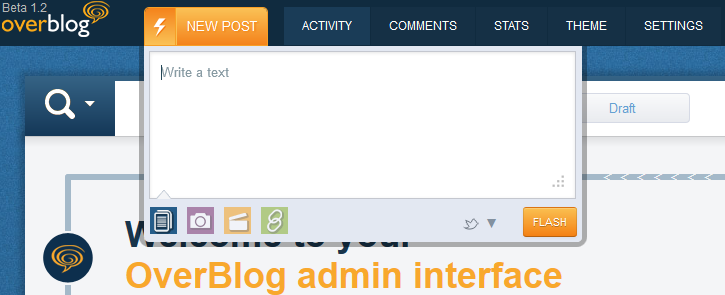
\includegraphics[width=13cm]{Images/flash001.png}
    \caption{Writing a basic post}
\end{figure}

Click the "FLASH" button at the bottom-right corner to publish this post when you are happy with it. 

\newpage
\subsubsection{Creating quality articles}

If you would like to start creating a good blog article, you should start using the "NEW POST" button to get acces to the advanced article editor with many useful features. 

\begin{figure}[H]
    \center
	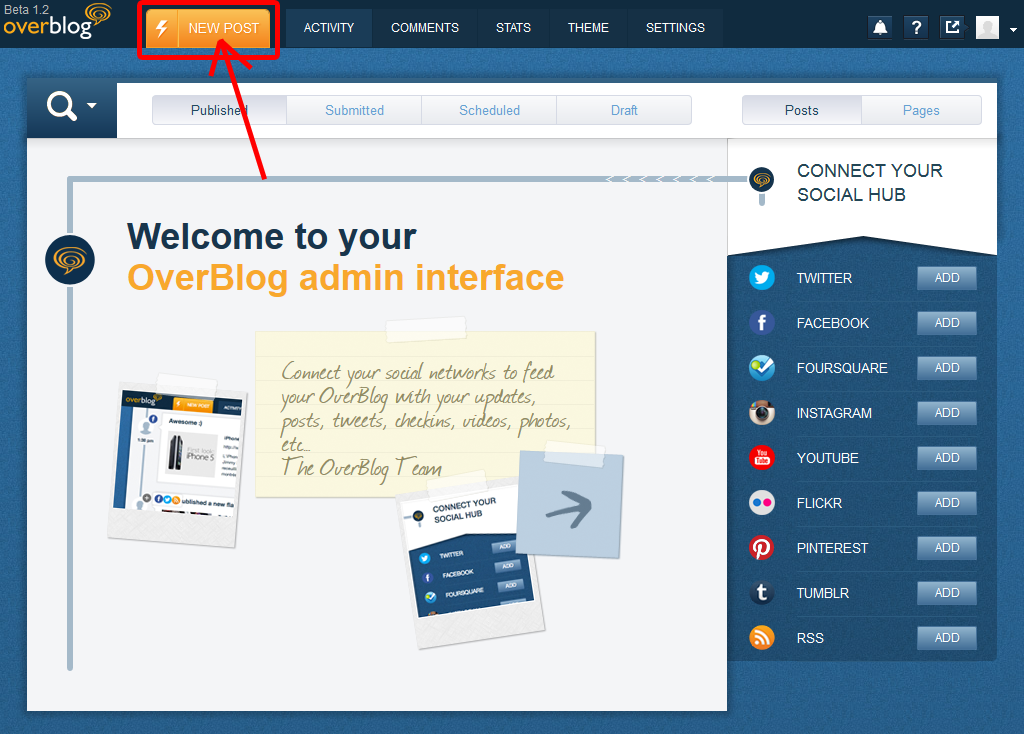
\includegraphics[width=12cm]{Images/newpostbutton001.png}
    \caption{Producing a real article}
\end{figure}

You have to give a main title to your article but keep in mind that it is important to find a good title to make your article sound intresting to the visitors of your blog. 

\begin{figure}[H]
    \center
	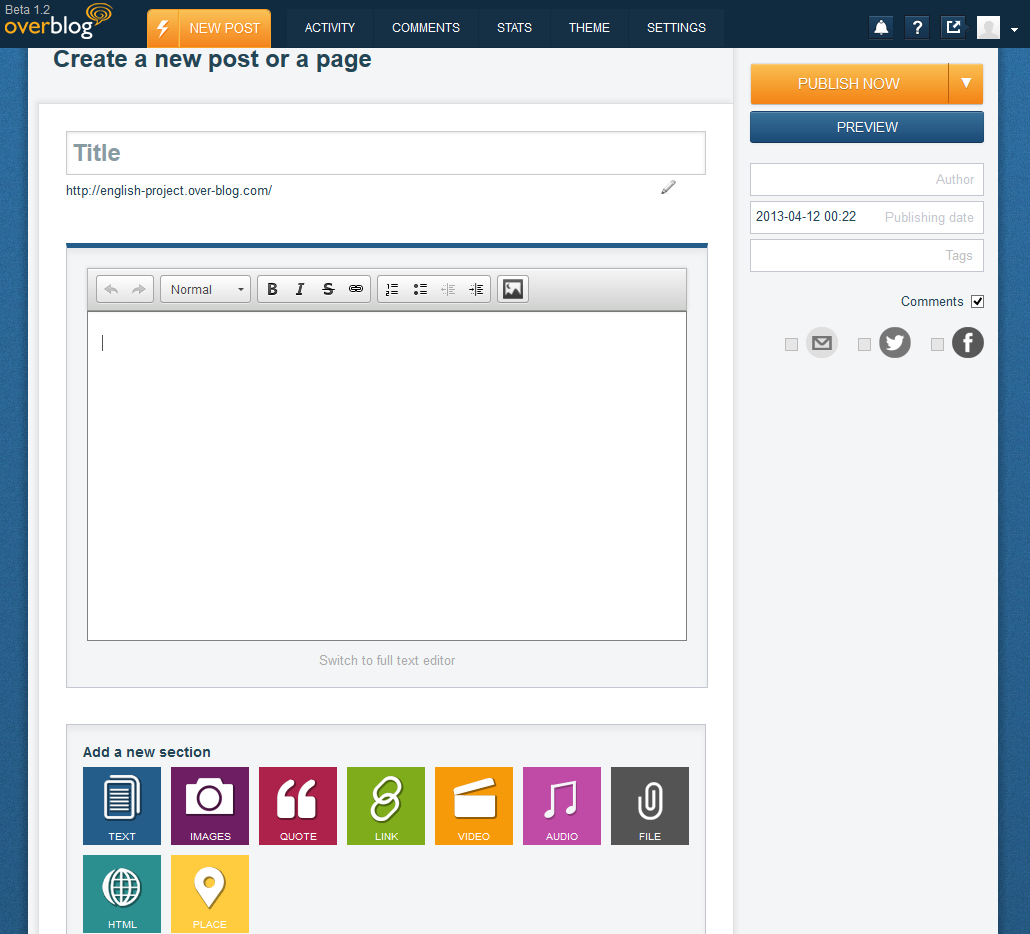
\includegraphics[width=10cm]{Images/article001.png}
    \caption{Building an article}
\end{figure}

Don't hesitate to structure your article with titles using the "format" selector to build the title hierarchy. Another useful feature for structuring your article is the possiblity of using lists ; these lists can be ordered or not. 

You can also emphasis the keywords in your text with the italic button. 

\newpage

\subsection{Articles and posts management}

When an article or a post is published or saved, it instantly apear in the posts/articles list. 

\begin{figure}[H]
    \center
	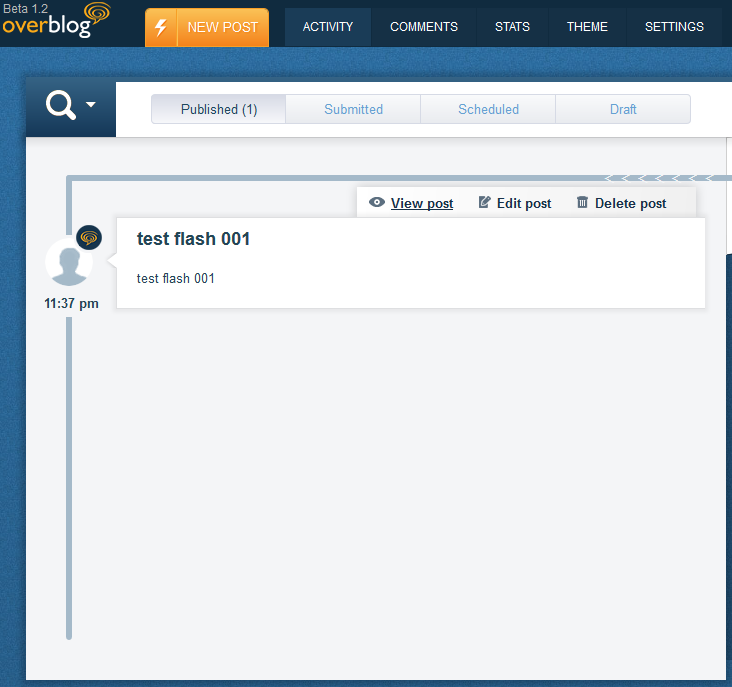
\includegraphics[width=10cm]{Images/view_edit_delete_001.png}
    \caption{Manage all the posts and articles listed below once created}
\end{figure}

By clicking "View post", you will be able to view the post/article as it is rendered on the pages of your blog for your visitors. 

If an article or a post needs revision, click the "Edit post" link to update the post/article or simply use the "Delete post" link to get rid of it. 

\begin{figure}[H]
    \center
	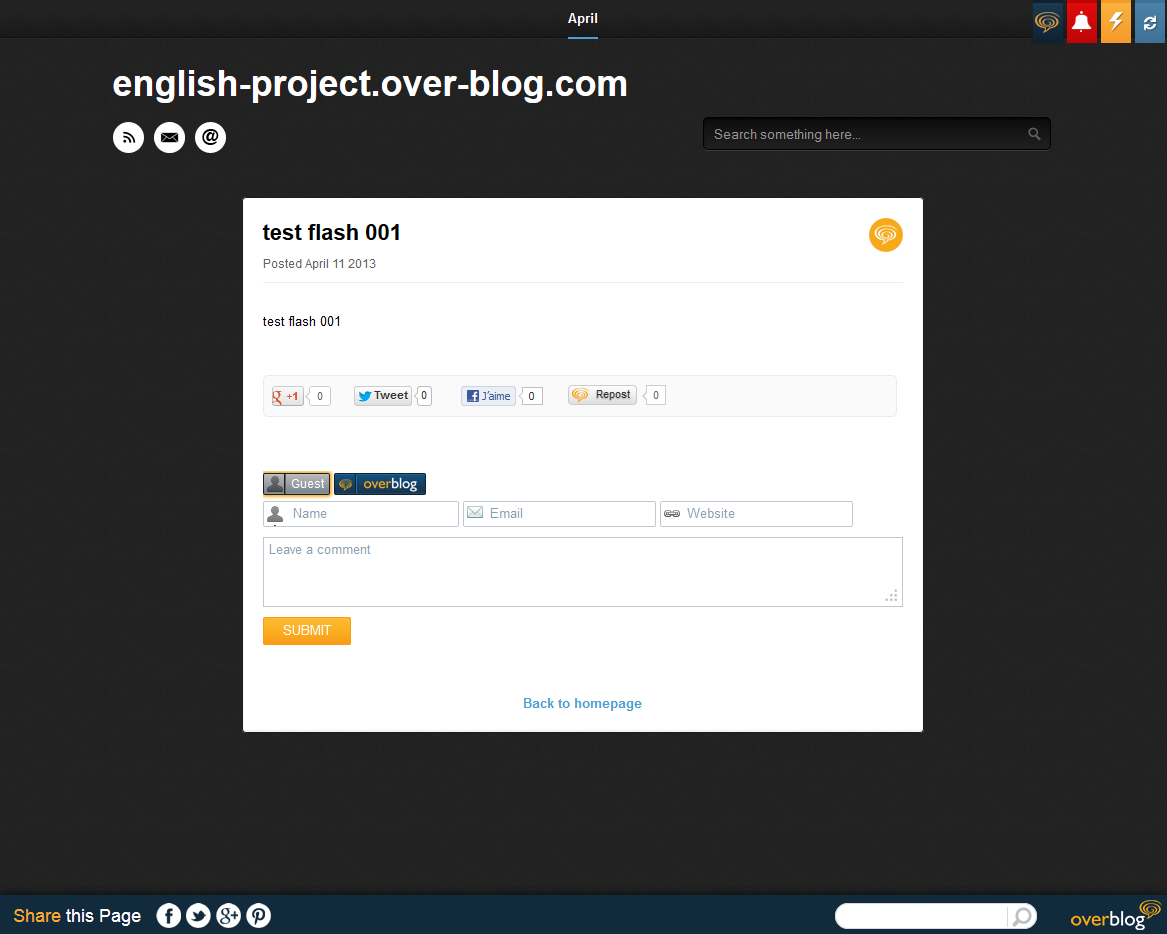
\includegraphics[width=10cm]{Images/view001.png}
    \caption{It is possible to watch the post or article through the eyes of a blog's anonymous visitor}
\end{figure}

\newpage

\subsection{Add some multimedia content}

Including a picture or a song to your article can just be with an illustration purpose, of course, but it would be great, if your article is about a photograph or a movie, to include an extract of it into the page to appeal the reader. 

\begin{figure}[H]
    \center
	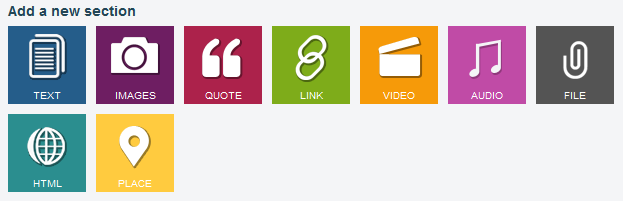
\includegraphics[width=10cm]{Images/multimedia001.png}
    \caption{It is possible to watch the post or article through the eyes of a blog's anonymous visitor}
\end{figure}

The multimedia features will allow you to include graphics, images, audio recordings, videos, files to share, internet links, geographical Points Of Interest and quotations. Advanced users can even include html parts of code for a better flexibility of the article. 

Feel free to discover all the tools given by the editor. The important is that the result will be worth the time spent on mastering the use of these tools. 

%%%%%%%%%%%%%%%%%%%%%%%%%%%%%%%%%%%%%%%%%%%%%%%%%%%%%%%%%%%%%%%%%%%%%%%%%%%%%
%%%%%%%%%%  Etape 3
%%%%%%%%%%%%%%%%%%%%%%%%%%%%%%%%%%%%%%%%%%%%%%%%%%%%%%%%%%%%%%%%%%%%%%%%%%%%%
\newpage

\section{Pimp your blog}
%TODO Guillaume
% Fond d’écran / catégorie / résumé
%personnalisation de base
\subsection{Basics}
With Overblog it is very simple to customize your blog. On the header, you can click on the theme button to access to theme customization page.
\begin{figure}[htpb]
 \centering
 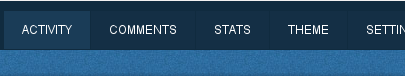
\includegraphics[scale=0.43]{Images/HeaderBar.png}
 \caption{Part of the header}
 \label{customHeader}
\end{figure}

When your are on the theme customization page, on the left panel you can see all the differents theme you can apply on your blog. There is something for
everyone... So when you select a theme you can see the preview, and to apply the theme you should click on the save button, or click on the cancel button if
you want to keep the previous theme.
\begin{figure}[htpb]
 \centering
 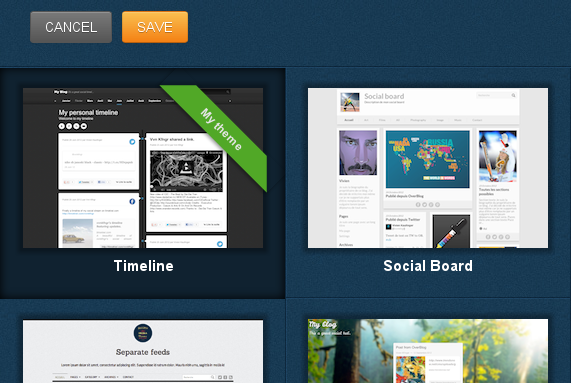
\includegraphics[scale=0.43]{Images/ChooseYourTheme.png}
 \caption{The theme chooser}
 \label{customHeader}
\end{figure}
%Personnaliser son blog sur overBlog est vraiment très facile. Sur la barre horizontal supérieur il y a un bouton thème (image du bouton)
%Sur le panneau sur la gauche de votre browser une liste de thème vous est proposé. il y en a pour tout les goûts...
%Le thème est appliqué sur la page d'aperçu pour permettre à M... de voir se que donnera le thème. Lorsque vous avez choisi le thème, il vous suffira de
% cliquer sur le bouton enregistrer(image du bouton) ou le bouton annuler (image du bouton) si au contraire M... souhaite garder le précédent thème.

%personnalisation avancée
\subsection{Advanced customization}
Overblog also provides a configuration for themes. these are not detailed in this document because there are many options. Moreover, these
options can be differents from one theme to another. It is also possible to modify the page html code directly and see the preview. It is discouraged to use
this mode except if you are a confirmed user.
% Overblog propose aussi un mode de configuration pour les thèmes. Je ne les détaillerais pas dans ce document, étant donné qu'il y a de très nombreuses
% options et que ces options peuvent être différentes d'un thème à l'autre. Il est même possible d'avoir et de modifier le contenu de la page html en direct et
% d'en avoir un aperçu. Je vous déconseille d'utiliser le mode html sauf si vous êtes un utilisateur confirmé.


%%%%%%%%%%%%%%%%%%%%%%%%%%%%%%%%%%%%%%%%%%%%%%%%%%%%%%%%%%%%%%%%%%%%%%%%%%%%%
%%%%%%%%%%  Etape 4
%%%%%%%%%%%%%%%%%%%%%%%%%%%%%%%%%%%%%%%%%%%%%%%%%%%%%%%%%%%%%%%%%%%%%%%%%%%%%
\newpage
\section{Sharing it}

\subsection{Social linkage}

The first time you come to the  \emph{Overblog admin interface} you cannot miss this Panel.
\begin{figure}[h]
    \center
  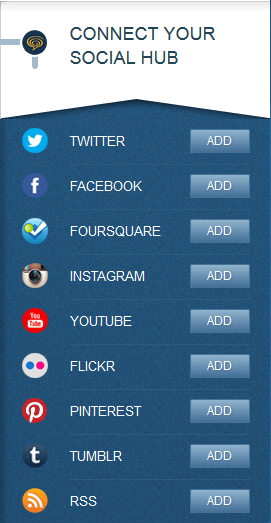
\includegraphics[width=0.3\textwidth]{Images/shareIni.png}
    \caption{Share panel}
\end{figure}

You can use it by clicking one of the buttons, like the Facebook button (if you have a Facebook account). Then agree with their proposal. With this linkage, you can feed your blog ! You are not obliged to rewrite your Facebook publications.

In another way, this linkage can allow your blog to ask your ``friends" to see your blog.

\subsection{Publish it on your favorite social networks !}

You can like your publications, or quote it by using the bar just under it.

\begin{figure}[h]
    \center
  
\includegraphics[width=0.9\textwidth]{Images/articleBar.png}
    \caption{Like bar}
\end{figure}

You are also able to share your article, even your blog, on your favorite social network. You just need to click on one of the following buttons.

\begin{figure}[h]
    \center
  
\includegraphics[width=0.5\textwidth]{Images/blogBar.png}
    \caption{Share bar}
\end{figure}

\subsection{Purpose}

But why do all that ? To make your friends come to see your blog, comment it, like it, and share it with their own friends ! So more and more people can come to your blog and see your kiwi jam ! So let's do it.

 


%%%%%%%%%%%%%%%%%%%%%%%%%%%%%%%%%%%%%%%%%%%%%%%%%%%%%%%%%%%%%%%%%%%%%%%%%%%%%
%%%%%%%%%%  CONCLUSION GENERALE
%%%%%%%%%%%%%%%%%%%%%%%%%%%%%%%%%%%%%%%%%%%%%%%%%%%%%%%%%%%%%%%%%%%%%%%%%%%%%
\newpage
\section{Conclusion}
So now you are ready to create your own blog and share it with all your friends.

And with all this knowledge, you are able to hack into FBI's system.

\end{document}

\begin{figure}[H]
    \center
    \subfloat[Boîte de dialogue pour le nom de la tâche]{\includegraphics[width=3.7cm]{Images/addTask.png}}\quad
    \subfloat[Tâche]{\includegraphics[width=3.7cm]{Images/listTask.png}}
    \caption{Ajout d'une tâche}
\end{figure}
